\newpage
\section{Decider for ``Translated cyclers''}\label{sec:translated-cyclers}

\begin{figure}[h!]
  \centering
  % 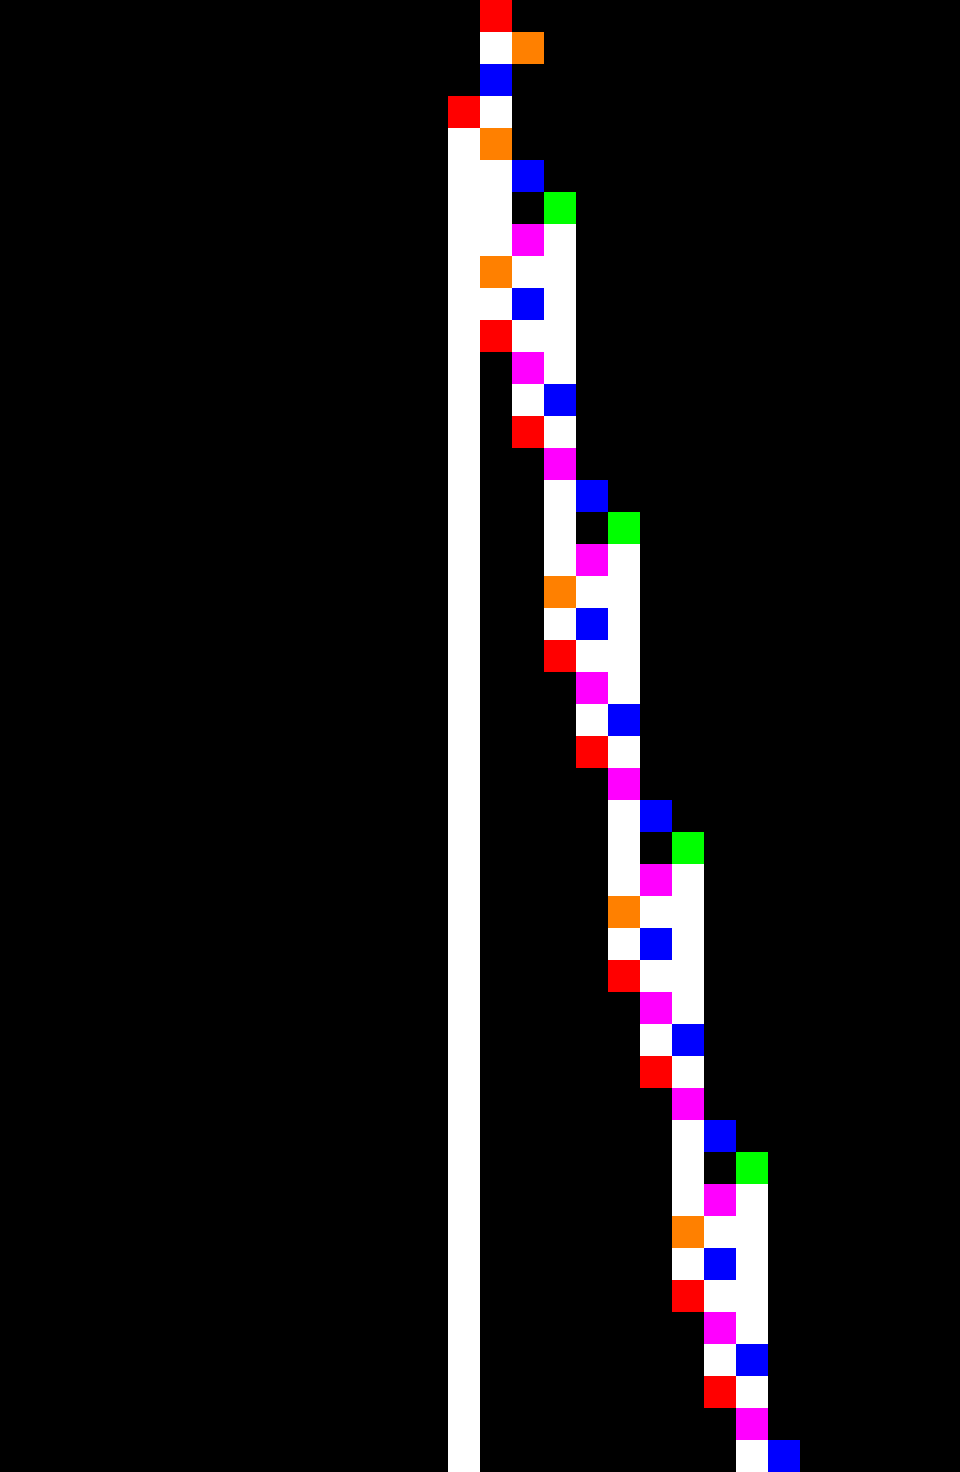
\includegraphics[width=0.5\textwidth]{space-time-diagrams/translated_cycler_44394115.pdf}
  % \hspace{2ex}
  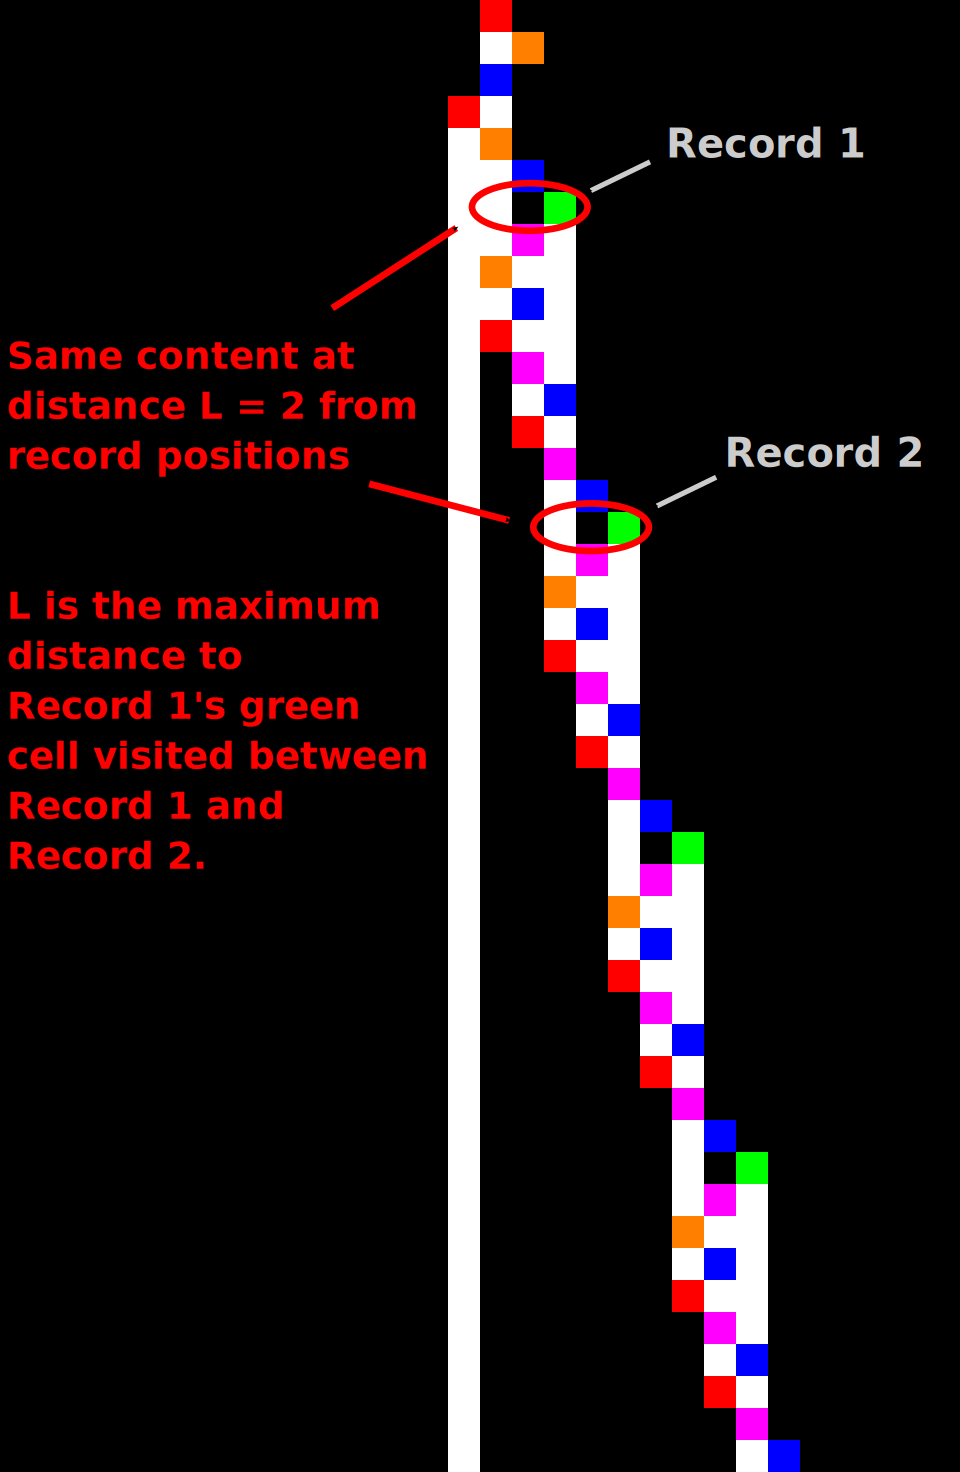
\includegraphics[width=0.54\textwidth]{space-time-diagrams/translated_cycler_44394115_annotated.pdf}

  \caption{Example ``Translated cycler'': 45-step space-time diagram of bbchallenge's machine \#44,394,115. See \url{https://bbchallenge.org/44394115}. The same bounded pattern is being translated to the right for ever. The text annotations illustrate the main idea recognising ``Translated Cyclers'': find two configurations that break a record (i.e. visit a memory cell that was never visited before) in the same state (here state \textcolor{colorD}{D}) such that the content of the memory tape at distance L from the record positions is the same in both record configurations. Distance L is defined as being the maximum distance to record position 1 that was visited between the configuration of record 1 and record 2.}\label{fig:translated-cyclers}
  \end{figure}
  
  The goal of this decider is to recognise Turing machines that translate a bounded pattern for ever. We call such machines ``Translated cyclers''. They are close to ``Cyclers'' (Section~\ref{sec:cyclers}) in the sense that they are only repeating a pattern but there is added complexity as they are able to translate the pattern in space at the same time, hence the decider for Cyclers cannot directly apply here.

  The main idea for this decider is illustrated in Figure~\ref{fig:translated-cyclers} which gives the space-time diagram of a ``Translated cycler': bbchallenge's machine \#44,394,115 (c.f. \url{https://bbchallenge.org/44394115}). The idea is to find two configurations that break a record (i.e. visit a memory cell that was never visited before) in the same state (here state \textcolor{colorD}{D}) such that the content of the memory tape at distance L from the record positions is the same in both record configurations. Distance L is defined as being the maximum distance to record position 1 that was visited between the configuration of record 1 and record 2. In those conditions, we can prove that the machine will never halt.

  The translated cycler of Figure~\ref{fig:translated-cyclers} features a relatively simple repeating pattern and transient pattern (pattern occurring before the repeating patterns starts). These can get significantly more complex, bbchallenge's machine \#59,090,563 is an example see Figure~\ref{fig:translated-cyclers-more} and \url{https://bbchallenge.org/59090563}. The method for detecting the behavior is the same but more resources are needed.


  
  \begin{figure}
  \centering
  % 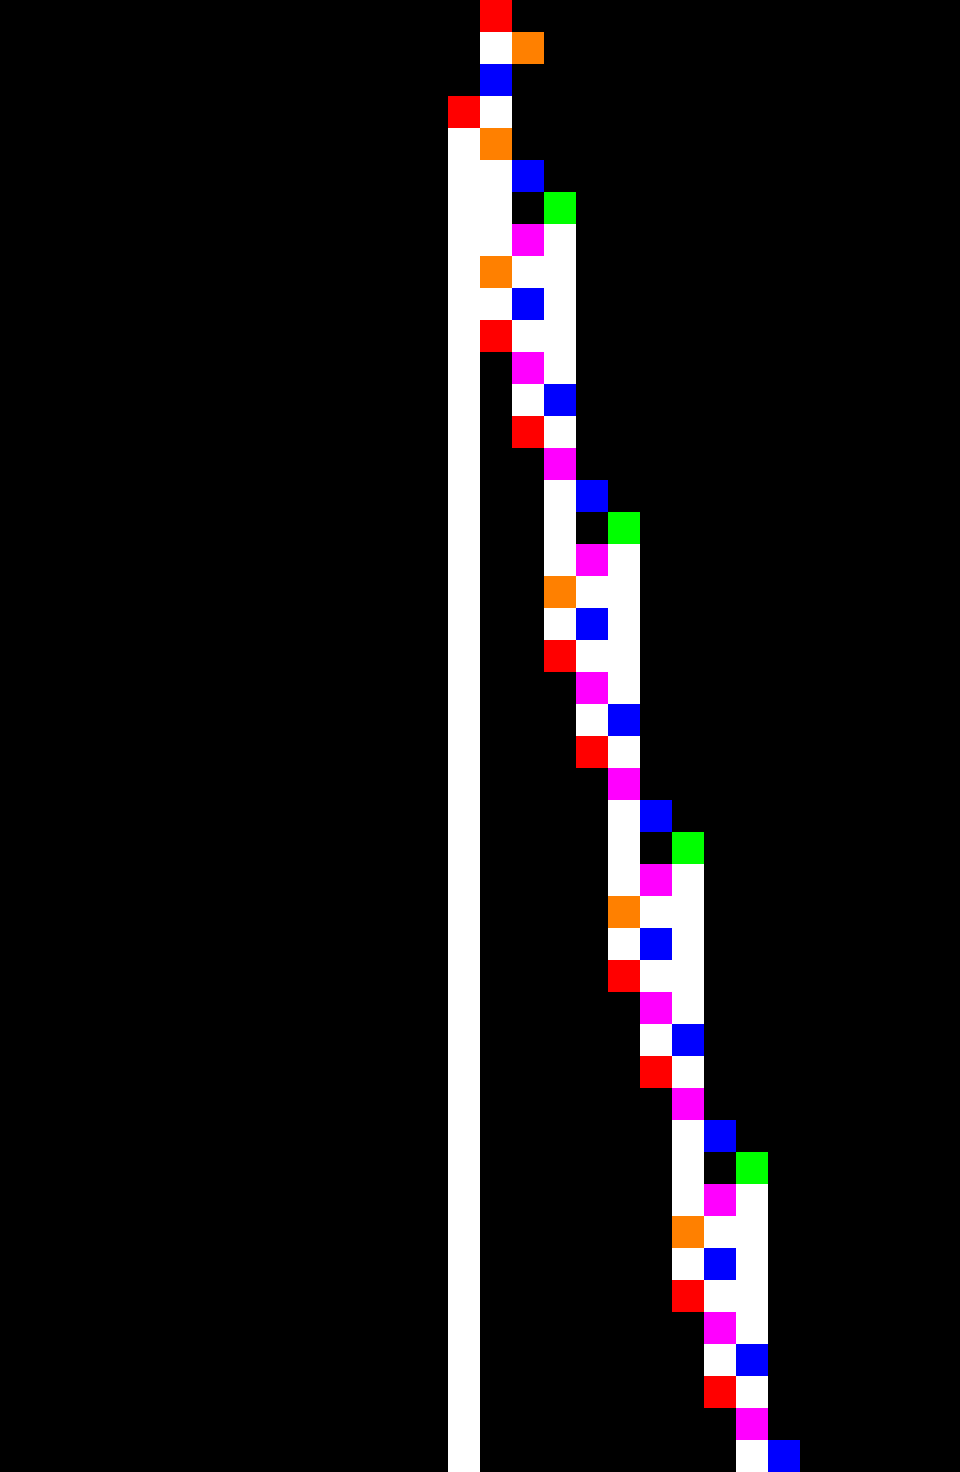
\includegraphics[width=0.5\textwidth]{space-time-diagrams/translated_cycler_44394115.pdf}
  % \hspace{2ex}
  \includegraphics[width=0.7\textwidth]{space-time-diagrams/translated_cycler_59090563.png}

  \caption{More complex ``Translated cycler'': 10,000-step space-time diagram (no state colours) of bbchallenge's machine \#59,090,563. See \url{https://bbchallenge.org/59090563}.}\label{fig:translated-cyclers-more}
  \end{figure}
  